\documentclass[{../../master}]{subfiles}
\graphicspath{{../../}}  % 個別コンパイル時の画像パスを解決する

\begin{document}

この章ではNavigation Stackによる自律移動を行うためのパッケージ作成について説明します.
Navigation Stackはその言葉の通り,移動ロボットの自律移動(Navigation)のための各種パッケージ群の集まりです.
移動ロボットの自律移動のためには,地図の読み込み,自己位置推定,目的地までのパス計画,パス追従,障害物検知等のアルゴリズムが必要です.
Navigation Stackはこれらの機能を提供しているため,これを使うことでオリジナルの移動ロボットに自律移動の機能を追加することができます.

% TODO: 本章の構成

\section{Navigation Stackの概要}

Navigation StackのROS Wikiのページ\footnote{\url{http://wiki.ros.org/navigation}}の概要文を引用してみましょう.

\begin{quote}
  A 2D navigation stack that takes in information from odometry, sensor streams, and a goal pose and outputs safe velocity commands that are sent to a mobile base.
\end{quote}

Navigation Stackは移動ロボットの2Dナビゲーションのためのメタパッケージです.
入力としてホイールオドメトリ,センサ(LiDAR,点群等)とゴール姿勢を受け取り,出力として安全な速度指定をロボットに与えます.

Navigation Stackのパッケージの関係図をROS Wikiから図\ref{fig:navigation_stack_overview}に引用します.

\begin{figure}[ht]
  \centering
  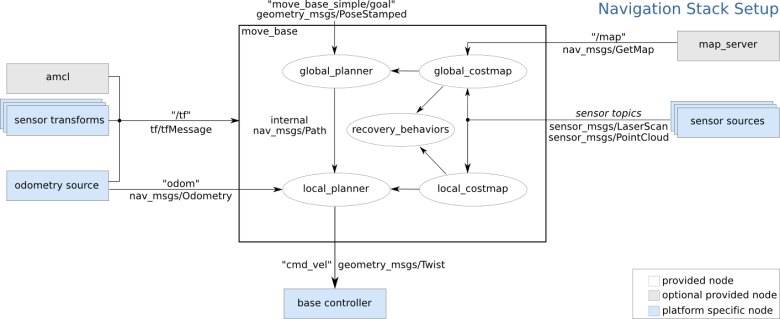
\includegraphics[width=120truemm]{images/navigation_stack_overview.png}
  \caption{Overview of Navigation Stack System}
  \label{fig:navigation_stack_overview}
\end{figure}

Navigation Stackはいくつかのパッケージから構成され,それぞれのパッケージが特定の機能を実現しています.
主なパッケージを以下に列挙します.

\begin{itemize}
  \item \textsf{move\_base} \\
    核となるパッケージです.パス計画,コストマップ,速度指令出力,復帰動作等を司ります.
    各機能を実現するアルゴリズムはプラグインの形で切り替えることができます.
  \item \textsf{amcl} \\
    センサとオドメトリからロボットの自己位置を推定します.
  \item \textsf{map\_server} \\
    SLAMによって作成・保存された地図データを各パッケージにトピックとして提供します.
\end{itemize}

独立したパッケージとして提供されているのは上の3つであり,ローカル・グローバルパスの計画を行うパッケージや障害物のコストマップを計算するパッケージは,\textsf{move\_base}パッケージのプラグインとして提供されています.
プラグインとしての主なパッケージは以下に挙げるものがあります.

\begin{itemize}
  \item \textsf{base\_local\_planner}:ローカルプランナの1つです.
  \item \textsf{dwa\_local\_planner}:ローカルプランナの1つです.
  \item \textsf{navfn}:グローバルプランナの1つです.
  \item \textsf{global\_planner}:グローバルプランナの1つです.
  \item \textsf{costmap\_2d}:コストマップを計算するパッケージです.
\end{itemize}

\textsf{move\_base}のプラグインはパラメータを指定することで簡単に切り替えることが可能になっています.

Navigation Stackを利用して自律移動機能を実装するには,オリジナルのロボットに合わせて各パッケージのパラメータを設定し,パッケージを起動してやる必要があります.
以降の節で,Navigation Stackの起動方法を説明していきます.

\end{document}